\documentclass[]{revdetua}
\usepackage{graphicx} % Required for inserting images

\Header{Volume}{14}{Novembro}{2023}{0}

\title{Advanced Algorithms - First Project \linebreak Maximum Clique Problem}
\author{Gonçalo Machado Nmec 98359}
\date{November 2023}

\begin{document}

\maketitle

\begin{abstract}
This report presents two algorithmic solutions for the Maximum Clique Problem, including a formal analysis of each algorithm's efficiency, a discussion of the obtained results, and predictions for large problem instances. This problem is addressed by the course "Advanced Algorithms" at the University of Aveiro. The proposed algorithms include one exhaustive search algorithm and one greedy algorithm that uses heuristics. The chosen coding language was Python.
\end{abstract}

\begin{resumo}% Note: in Portuguese
Este relatório apresenta duas soluções algorítmicas para o problema Clique Máximo, incluindo uma análise formal da eficiência de cada algoritmo, uma discussão dos resultados obtidos e previsões para problema de maior escala. Este problema é abordado pelo curso "Algoritmos Avançados" na Universidade de Aveiro. Os algoritmos propostos incluem um algoritmo de pesquisa exaustiva e um algoritmo guloso que utiliza heurísticas. A linguagem de programação escolhida foi Python.
\end{resumo}

\begin{keywords}
Graph, Clique, Maximum Clique, Edges, Vertices, Exhaustive Search, Greedy Algorithm, Heuristics
\end{keywords}

\begin{palavraschave}
Grafo, Clique, Clique Máximo, Arestas, Vértices, Pesquisa Exaustiva, Algoritmo Guloso, Heurísticas
\end{palavraschave}

\section{Introduction}
This reports is part of the first project of "Advanced Algorithms". The goal of the project was to design and test two algorithms, one that used exhaustive search and other that used greedy heuristics, to solve the \textbf{Maximum Clique} problem.

The following sections describe the problem and some key concepts, explain how the graphs were created, how each algorithm works and analyse the performance and computation complexity of the algorithms. For the analysis, both a formal computational analysis and an experimental computational analysis were done, with the latter consisting of a series of experiments, for successively larger problem instances, where the \textbf{number of basic operations}, the \textbf{execution time} and the \textbf{number of solutions / attempts tested} were registered. The analysis were compared with each other and an attempt to estimate the execution time of the algorithms for much larger problem instances was made.

Alongside the report there were also the files containing the code developed, the graphs used in the experiments and the results derived from the code. In order to run the code, we first generate the graphs, then run the file with the chosen algorithm. The commands used to run the code are the following: \linebreak

\$ python generate\_graphs.py 

\$ python exhaustive\_search.py

\$ python greedy\_heuristics.py

\section{Maximum Clique Problem}

As said before, the goal of the project was to solved the \textbf{Maximum Clique Problem}, which asks us to find a maximum clique for a given undirected graph G(V, E), with n vertices and m edges. A clique of G is a subset of vertices, all adjacent to each other, i.e., defining a complete subgraph of G. A maximum clique is a clique with the largest possible number of vertices. Example: in a social network, a clique is a subset of people who all know each other.

An important fact is that a graph can have more than one maximum clique, which happens if there are two cliques with the same size and there are no cliques with bigger size than them. In this case, the algorithms will return one of the maximum cliques.

The problem given to us also described the characteristics of the graph instances that would be used by the algorithms, which are the following:

\begin{itemize}
\item Graph vertices are 2D points on the XoY plane, with integer-valued coordinates between 1 and 100.
\item Graph vertices should neither be coincident nor too close.
\item The number of edges sharing a vertex is randomly determined.
\item Use 12.5\%, 25\%, 50\%, and 75\% of the maximum number of edges for the number of vertices.
\item Graph edges are unweighted and undirected.
\item The graphs need to be generated using a student number as the seed.
\end{itemize}

To construct a graph, and following the rules given to us, we first need to generate the list of vertices. Each vertex has a randomly generated tuple of integer-valued coordinates between 1 and 100 and an ID associated to them. One of the rules states that the vertices should neither be coincident nor too close, and while the first part is certain ( two vertices are either coincident or not), the second part is subjective to interpretation. As such, we considered that two vertices were "too close" if the distance between them was less than 7. Before being added to the list, each vertex was compared to every other vertex to check if the distance was below the minimum defined. For this problem we decided that the number of vertices of a graph would be between 4 and 150, since more than this would not be feasible for the algorithms to use.

After generating the list of vertices, we need to generated the list of edges. One of the rules states that a percentage of the maximum number of edges needs to be used when generating the list, so for each number of vertices in a graph, we created 4 graphs, each using a different percentage of the maximum number of edges. The maximum number of edges is calculated with the formula: \( n(n-1)/2 \) where n is the number of vertices in the graph. Each edge is generated by randomly picking two vertices and seeing if an edge between the two exists, and if not, add a tuple with the ids of the two vertices to the list of edges.

After generating each graph, and in order to store them for later use, we create a JSON with two fields:

\begin{itemize}
    \item vertices - Contains a JSON object where each pair has the id of the vertex as the key and the coordinates as the value
    \item edges - Contains a list of edges, with each edge being a list of the ids of the two vertices that the edge is connected to.
\end{itemize}

The object is then saved with a name that follows the format {number of vertices}\_vertices\_{percentage of maximum edges}\_edge\_percentage. An example of the object would be:
\linebreak \linebreak
 \{"vertices": {"0": [20, 70], "1": [72, 75], "2": [48, 23], "3": [48, 52], "4": [74, 43]}, "edges": [[1, 0], [4, 1], [4, 2], [1, 2], [4, 0]]\}
\linebreak

To load the graph we simply read the content of the JSON and using \textit{Networkx} create a networkx.Graph object and insert each vertex and each edge into the object.

After using an algorithm to get the maximum cut of the graph, we obtain a maximum clique of the graph, which consists in a list of the ids that are in the maximum clique. For example, the maximum clique of the graph used in the previous example is [0,1,4].

\section{Analysis of Algorithm Efficiency}

To analyse the efficiency of an algorithm, we will do so as a function of the algorithm's input size. In our case, it is the size of list of vertices in the generated graphs.

As per requested in the problem given to us, we will use the \textbf{number of basic operations}, the \textbf{execution time} and the \textbf{number of solutions / attempts tested} to measure the algorithm's efficiency. From these three values, it is worth mentioning that the execution time is not the best parameter to use in order to assess the efficiency, since it largely depends on the machine were the algorithm is ran, the language the algorithm was written on and the use or not of parallelization.

The \textbf{number of basic operations} is the best parameter to analyse the efficiency, since it does not depend on external factors, it only depends on the algorithm itself. A basic operation is the operation contributing the most to the total running time of an algorithm usually being the most time consuming operation in the algorithm's innermost loop. The basic operation of each algorithm will be described in the sections of the algorithms.

When analysing the efficiency of an algorithm, we should also understand that the algorithm might have different number of basic operations for graphs of the same input size. Due to this, we will consider:

\begin{itemize}
    \item Worst-case scenario - The worst-case efficiency of an algorithm is its efficiency for the worst-case input of size n (for which the algorithm runs the longest among all possible inputs of that size)
    \item Best-case scenario - The best-case efficiency of an algorithm is its efficiency for the best-case input of size n (for which the algorithm runs the fastest among all possible inputs of that size)
\end{itemize}

Each of the cases will be addressed with more detail in the sections pertaining each algorithm.

\section{Exhaustive Search Algorithm}

An exhaustive search algorithm is a brute-force algorithm that systematically enumerates all possible solutions to a problem and checks each one to see if it is a valid solution. This kind of algorithm is typically used when the search space is small and well defined because checking all possible solutions in a large space will take a large amount of time, and when the space is not well defined the search can't be done accurately and systematically.  

The algorithm first loads all graphs that will be used, which in our case includes graphs with a number of vertices between 4 and 30. Then the algorithm gets the adjacency matrix of the graph, which will be used to get the maximum clique. An adjacency matrix is a matrix containing rows and columns which is used to represent a simple labelled graph, with 0 or 1 in the position of (\textit{Vi} , \textit{Vj}) according to the condition whether \textit{Vi} and \textit{Vj} are adjacent or not. 

Using the adjacency matrix and the list of vertices, the algorithms creates all combinations of vertices without repetition with size n  where n is the size of the list of vertices and checks if the combination of vertices is a clique. If the combination is a clique, it returns the combination as well as the number of basic operations performed and the number of attempts tested. If the combination is not a clique, it continues to check the combinations of size n, and if none of them are a clique, it creates the combinations of size n-1, and so on, until the combinations have only 1 vertex, meaning that the graph is disconnected or, in other words, has no edges between vertices, returning a combination with only 1 vertex, as well as the number of basic operations and the number of attempts tested.

The basic operation of this algorithm is the act of checking if a combination is a clique using the adjacency matrix. Since this algorithm starts with combinations of vertices of the maximum size possible (which is the graph itself) and gradually decreases the size of the combinations until it finds a clique, the first clique found will be a maximum clique of the graph, and there is no reason to test all the other combinations. As such, there are best-case, worst-case and average-case cenarios in the algorithm.

The best-case scenario is when the graph itself is a clique, meaning that the algorithm will only perform 1 operation. In this case, the algorithm has an time complexity of O(1).

The worst-case scenario is when the graph is disconnected, meaning that the maximum clique is composed of a single vertex. In this case, the algorithm will check all combinations possible, which are \( 2^n \), making the complexity O(\( 2^n \)).

To note that the number of solutions tested is equal to the number of basic operations done, since only one basic operations is done per solution tested.

From the previous assessments, we can see that the algorithm, although simple, has a great cost in terms of time complexity, with the worst-case scenario having a complexity of O(\( 2^n \)). We can conclude that the algorithm's order of growth is exponential, and the larger problem instance the higher the number of basic operations.

The exhaustive algorithm was ran for a full night and reached a maximum of 33 vertices with a time of 4291 second, which is an hour and 11 minutes. The algorithm was able to get the solution in under 60 seconds for a graph with 27 vertices.

\section{Greedy Algorithm}

The second algorithm developed was greedy algorithm that uses heuristics. A greedy algorithm is any algorithm that follows the problem-solving heuristic of making the locally optimal choice at each stage. 

This algorithm starts by loading all graphs that will be used, with the graphs containing anywhere between 4 and 150 vertices. The algorithm then gets the adjacency matrix of the graph, which will use to get the maximum clique in the graph. It does this by starting with an empty set and iteratively adding vertices to it, ensuring that the current set remains a clique. The clique obtained by this algorithm is not necessarily the maximum clique of the graph, which derivates from the nature of using heuristics and not checking every possibility.

The algorithm basic operation is where it checks if adding the vertex to the current set does not affect the set being considered a clique. Since we iterate over every vertex, the number of basic operations done will be the same as the input size, and since one basic operation is done per solution tested, the number of solutions tested will also be the same as the number of basic operations done. Another consequence of this fact is that there are not best-case or worst-case scenario, since it will iterate over every vertex.

The algorithm performs relatively well (time and space-wise) since it the number of basic operations needed grows at the same rate as the input size, but as stated before, it does not guarantee the return the maximum clique. The complexity of the algorithm is O(n).

\section{Results}

\subsection{Experiments}

For the experiments of both algorithms, graphs with vertices between 4 and 150 vertices and 12.5\%, 25\%, 50\%, and 75\% of the maximum number of edges for the number of vertices were used. Although the greedy algorithm was able to return a maximum clique for every graph, the exhaustive search as stated before only gave a solution for a graph with 33 vertices with an execution time of 1 hour and 11 minutes.

When comparing the size of the maximum cuts given to us by both algorithms for the same graph, and with the premises that the exhaustive search algorithm always returns a maximum clique of the graph and that a graph can have more than one maximum clique as long as they have the same size and there is no clique with a bigger size, we see that the accuracy of the greedy algorithm was 37.8\%. 

\subsection{Basic Operations}

\begin{figure}[h]
    \centering
    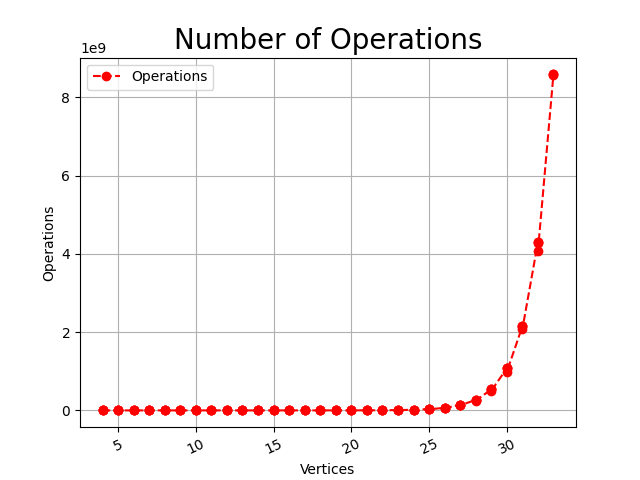
\includegraphics[width=8cm]{operations_exhaustive.png}
    \caption{Exhaustive Search Basic Operations}
\end{figure}

\begin{figure}[h]
    \centering
    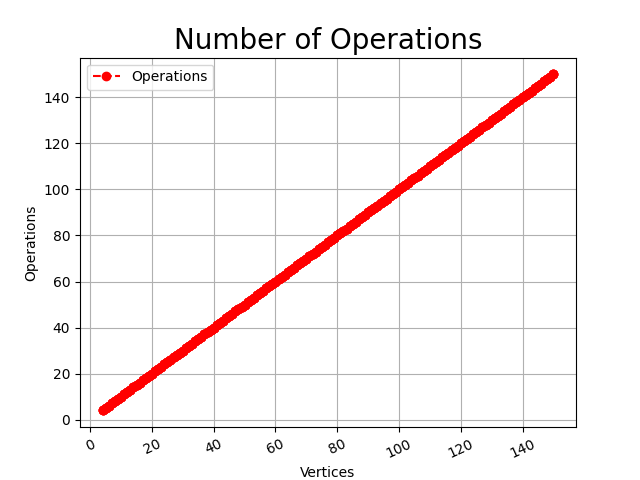
\includegraphics[width=8cm]{operations_greedy.png}
    \caption{Greedy Algorithm Basic Operations}
\end{figure}

By looking at the previous graphs, the experimental analysis is on pair with the formal analysis:

\begin{itemize}
\item The exhaustive algorithm's order of growth is exponential.
\item The greedy algorithm's order of growth is linear.
\end{itemize}

\subsection{Attempts Tested}

\begin{figure}[h]
    \centering
    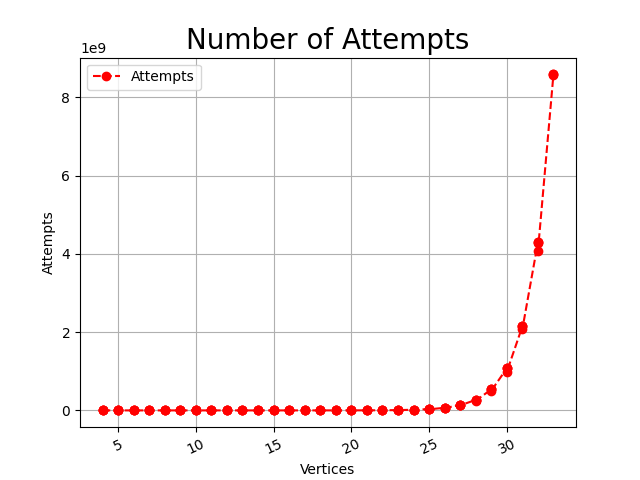
\includegraphics[width=8cm]{attempts_exhaustive.png}
    \caption{Exhaustive Search Attempts}
\end{figure}

\begin{figure}[h]
    \centering
    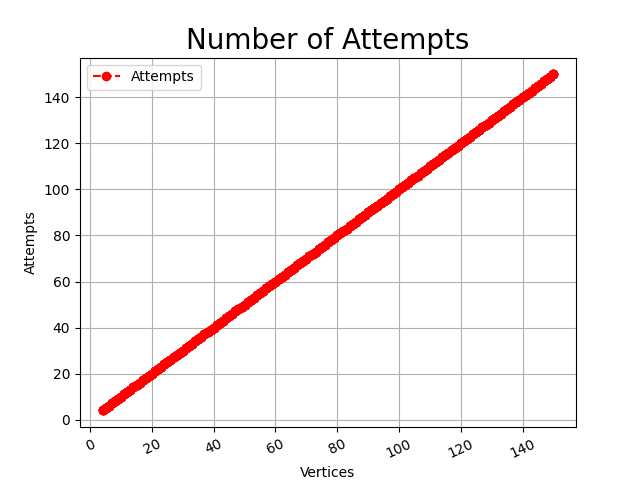
\includegraphics[width=8cm]{attempts_greedy.png}
    \caption{Greedy Algorithm Attempts}
\end{figure}

Once again, we were able to prove empirically what we concluded in the formal analysis:

\begin{itemize}
\item For both algorithms, the number of solutions tested is the same as the number of basic operations.
\end{itemize}

\subsection{Execution Time}

\begin{figure}[h]
    \centering
    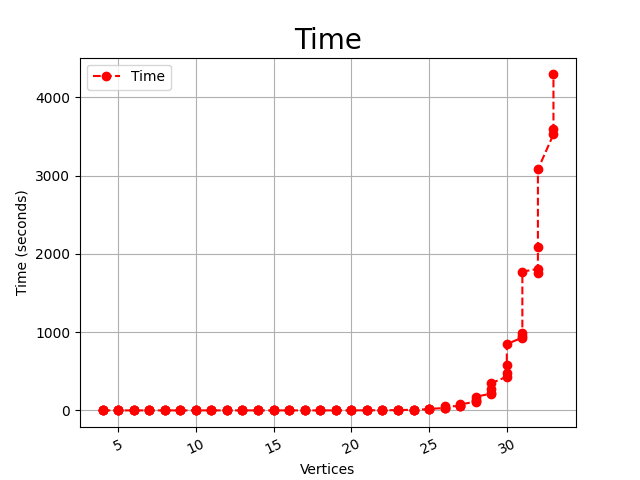
\includegraphics[width=8cm]{time_exhaustive.png}
    \caption{Exhaustive Search Execution Time}
\end{figure}

\begin{figure}[h]
    \centering
    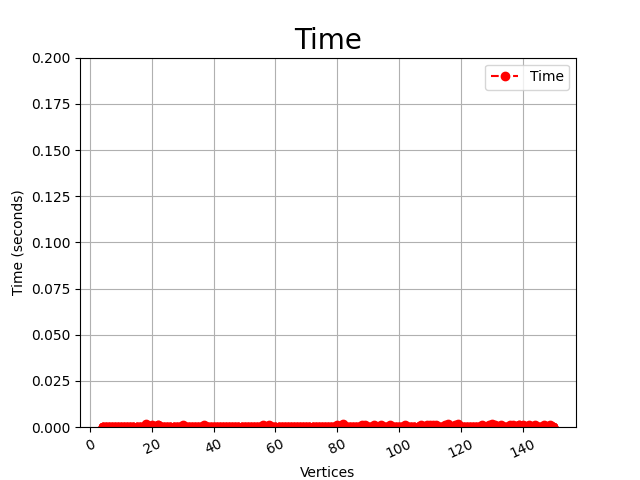
\includegraphics[width=8cm]{time_greedy.png}
    \caption{Greedy Algorithm Execution Time}
\end{figure}

When analysing the graphs related to the execution time in seconds, we can take some conclusions:

\begin{itemize}
    \item For the exhaustive search, the time grows at an exponential rate, which matches with the formal analysis
    \item For the greedy algortihm, the time in most of the situations is 0 seconds or very close to 0. This goes against the formal analysis that predicted that the algorithm would have a linear growth of time in function of the input size.
\end{itemize}

\section{Conclusion}

In conclusion, while the exhaustive search always reaches an optimal solution, it is very expensive in terms of complexity, due to its exponental growth. On the other hand, the greedy search is very cheap complexity and time wise, the result might not be the optimal solution, but instead an local optimal solution. This shows the balance that is usually associated with algorithms between complexity and optimal results.

\begin{thebibliography}{00}

\bibitem{b1} Wikipedia (2023). \textit{Maximal clique} [Online]. Available: \url{https://en.wikipedia.org/wiki/Clique_problem#:~:text=%5Bedit%5D-,Finding%20a%20single%20maximal%20clique,-%5Bedit%5D}
\bibitem{b2} Wolfram Alpha \textit{Maximal clique Problem} [Online]. Available: \url{https://mathworld.wolfram.com/MaximalClique.html}

\end{thebibliography}

\end{document}